\subsection{Eliminar elemento}

  \paragraph{}Para eliminar un elemento del sistema,  es necesario pulsar el
  icono \textit{Eliminar}. Se puede ver una captura de pantalla de este
  icono en la figura \ref{capturaDelElemento}.

  \begin{figure}[!ht]
    \begin{center}
      \fbox{
      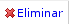
\includegraphics[scale=0.6]{3.Caracteristicas_Interfaz/3.3.Gestion_Informacion/3.3.4.Eliminacion_Elementos/delElemento.png}
      }
      \caption{Captura de pantalla del icono \textit{Eliminar}.}
      \label{capturaDelElemento}
    \end{center}
  \end{figure}

  \paragraph{}Al pulsar en el icono, se enlazará con la ventana de confirmación
  para eliminar el elemento. Esta ventana se puede ver en la imagen
  \ref{capturaConfirmacion}.

  \begin{figure}[!ht]
    \begin{center}
      \fbox{
      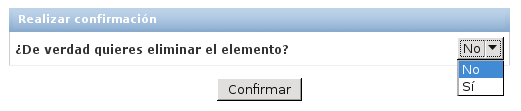
\includegraphics[scale=0.6]{3.Caracteristicas_Interfaz/3.3.Gestion_Informacion/3.3.4.Eliminacion_Elementos/pantalla_confirmacion.png}
      }
      \caption{Captura de pantalla de la ventana de confirmación para \textit{Eliminar} un elemento.}
      \label{capturaConfirmacion}
    \end{center}
  \end{figure}

  \paragraph{}Una vez realizada la confirmación, se pulsará el botón
  \textit{Confirmar}, el cual se puede ver en la figura
  \ref{capturaBotonConfirmar}. Si hemos elegido \textit{Sí} en la lista
  desplegable, el elemento se eliminará del sistema. Si por el contrario hemos
  elegido \textit{No}, se cancelará la eliminación del elemento y se devolverá
  al usuario a la lista del elemento.
